The following document specifies the calls that the Peer Manager Year3 Proof of Concept accepts and the replies (example+format) that it produces.
This is a work in progress, new calls may be added but the already specified calls should remain stable

\subsection{Creation of a new Peer}
This call will create a peer structure, its corresponding main entity (based on the peer\_type argument) and a user structure (with the given username) linked to the peer. 
CALL format

\begin{figure*}[htb!]
\centering
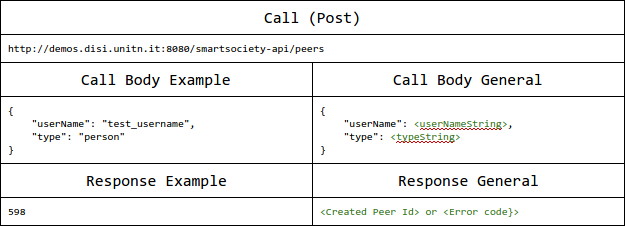
\includegraphics[width=1\linewidth]{figures/abs-new-peer.png}
\label{fig:abs-new-peer}
\end{figure*}

PARAMETERS
\begin{itemize}
	\item userNameString(required): alphanumeric string containing an unique username
	\item typeString(required): one of the following strings "human", "software"
\end{itemize}

POSSIBLE ERROR RETURNS (to be finalized)
\begin{itemize}
	\item NAME\_TAKEN: the provided username was already taken in the system
	\item INVALID\_TYPE: the provided type is not supported
\end{itemize}

\subsection{Update Peer Information}
This call updates the information in the main entity of the recently created peer.

\begin{figure*}[htb!]
\centering
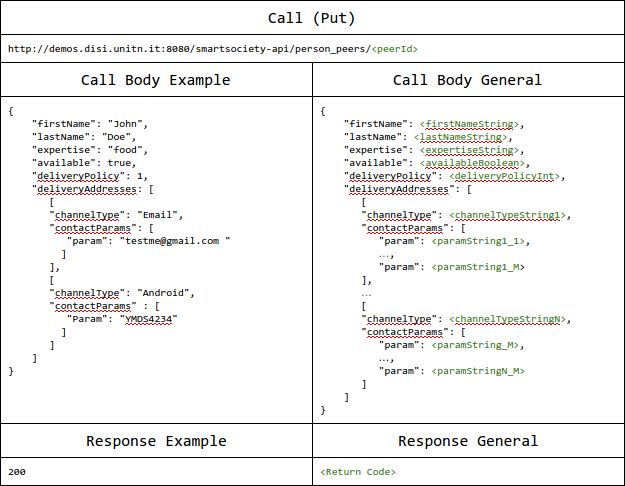
\includegraphics[width=1\linewidth]{figures/abs-update-peer.png}
\label{fig:abs-update-peer}
\end{figure*}

PARAMETERS
\begin{itemize}
	\item peerId (required - part of the call): id of the peer to update
	\item firstNameString(required): alphanumeric string containing first name of the represented person 
	\item lastNameString(required): alphanumeric string containing last name of the represented person
	\item expertiseString alphanumeric string (parsed later to a concept) that denotes the particular expertise of this person
	\item availableBoolean(required): boolean value that codifies if this peer is available for answering requests
	\item deliveryPolicyInt(required): integer value that codifies whether to deliver the message to one or more defined delivery Addresses (see SmartCom for the meaning of values, no validation done in the PM).
	\item channelTypeStringX(at least one required): string value that codifies the type of the communication channel  (see SmartCom for the meaning of values, no validation done in the PM)
	\item paramStringX\_Y(at least one required): string value that codifies a parameter that is useful for the current delivery address (e.g. the email address for an email type delivery address)
\end{itemize}

POSSIBLE ERROR RETURNS (to be finalized)
\begin{itemize}
	\item OK: peer updated without problem
	\item NOT\_A\_PERSON: the identified peer does not have a person main entity
	\item DATA\_INVALID: there was a problem processing the call body
\end{itemize}

\subsection{Create a SmartAsk Expert Profile}
This call updates creates a SmartAsk Profile for a given user\_id, this denotes that the user is in fact granting permission to SmartAsk to use the information contained in the profile.

\begin{figure*}[htb!]
\centering
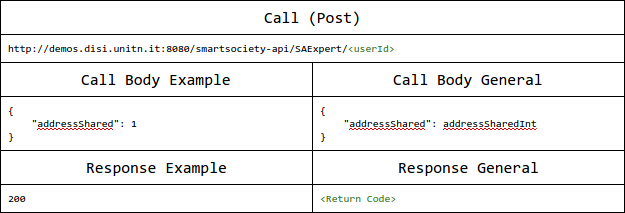
\includegraphics[width=1\linewidth]{figures/abs-new-profile.png}
\label{fig:abs-new-profile}
\end{figure*}

PARAMETERS
\begin{itemize}
	\item user\_Id (required - part of the call): id of the user of which to create the SAExpert profile
	\item addressShared: order of the delivery address that wants to be included in the created profile (1 means the first one defined, 2 the second, and so on). Defaults to 1
\end{itemize}

POSSIBLE ERROR RETURNS (to be finalized)
\begin{itemize}
	\item OK: profile created without problem
	\item INVALID\_USER: there user id was not found or does not belong to the authenticated user.
	\item INVALID\_ADDRESS: the address number was not defined
\end{itemize}